\documentclass[a4paper]{article}

\usepackage{graphicx}
\usepackage{amsmath,amssymb}
\usepackage{minted}
\usepackage{multirow}
\usepackage{float}
\usepackage{todonotes}
\usepackage{forest}
\usepackage{xstring}
\usepackage{xcolor}
\usepackage[most]{tcolorbox}
\usepackage{xparse}
\usepackage{natbib}

\usetikzlibrary{graphs,graphdrawing}
\usegdlibrary{layered}

% for external graphviz
\input{/home/donkarlo/Dropbox/repo/nd_ai_project/src/nd_ai/knoweldge_representation/language/formal/computer/programming/tex/latex/code_clips/external_graphviz.tex}

% for tags
\input{/home/donkarlo/Dropbox/repo/nd_ai_project/src/nd_ai/knoweldge_representation/language/formal/computer/programming/tex/latex/parts/control_sequence/kind/semtag/semtag.tex}

% for links
\input{/home/donkarlo/Dropbox/repo/nd_ai_project/src/nd_ai/knoweldge_representation/language/formal/computer/programming/tex/latex/code_clips/seehere.tex}

\title{Memory}
\date{}

\begin{document}
    \maketitle
    \section{Definition}
    Memory is the faculty of the mind by which data or information is encoded, stored, and retrieved when needed. It is the retention of information over time for the purpose of influencing future action. \seeherefooter{https://en.wikipedia.org/wiki/Memory}
    
    
    Most refrences such as~\cite[p.~3]{slotnick-2017-cognitive-neuroscience-of-memory}consider mental memory structure as a tree as follows
    \begin{figure}[H]
        \centering
        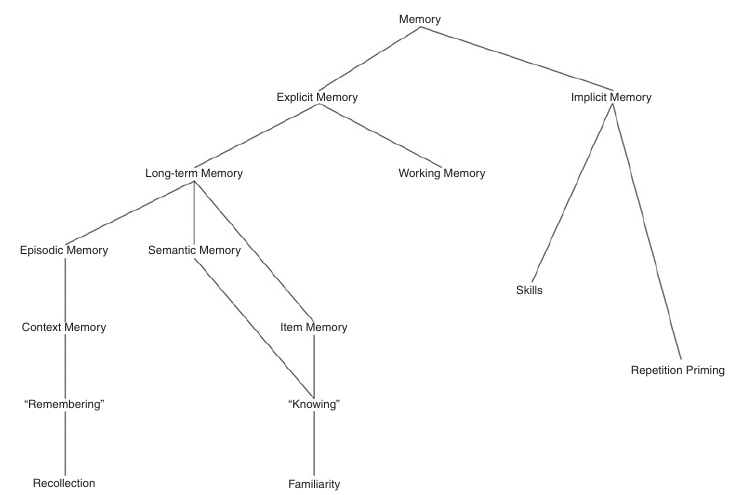
\includegraphics[width=0.9\textwidth]{slotnick-2017-cognitive-neuroscience-of-memory-figure-1-2}
        \caption{\cite{slotnick-2017-cognitive-neuroscience-of-memory} Fig. ~1.2}
    \end{figure}
    
    \bibliographystyle{plainnat}
    \bibliography{/home/donkarlo/Dropbox/repo/nd_shared_research/bibliography/bibliography.bib}
\end{document}